\documentclass{article}
\usepackage{amsmath}
\usepackage{amssymb}
\usepackage{geometry}
\usepackage{booktabs}
\usepackage{graphicx}
\usepackage{hyperref}
\usepackage{float}

\geometry{a4paper, margin=1in}

\title{\textbf{EE2801 - DSP LAB \\ EXPERIMENT-3} \\ Fixed-Point Division using Newton-Raphson iterations}
\author{EE24BTECH11012 - BHAVANISANKAR G S}
\date{\today}

\begin{document}

\maketitle

\tableofcontents

\newpage
\section{Aim}
To perform fixed point division by the method of Division by Reciprocation using Newton-Raphson method. The initial guess for Newton-Raphson method has been done in three ways - 
\begin{itemize}
    \item The optimal unconstrained linear minimax approximation.
    \item The hardware-constrained linear approximation (slope fixed to 2).
    \item The quadratic minimax approximation.
\end{itemize}

\section{Newton-Raphson Method for Reciprocation}

Given a continuously differentiable function $f(x)$ and a current approximation $x_n$ near the true root, we can approximate the curve of the function by its tangent line at the coordinate $(x_n, f(x_n))$. The slope of the tangent line at this point is given by the derivative, $f'(x_n)$. Using the point-slope form of a linear equation, the equation for this tangent line is:
\begin{equation}
    y - f(x_n) = f'(x_n)(x - x_n)
\end{equation}

The algorithm assumes that the $x$-intercept of this tangent line provides a better approximation of the true root than $x_n$. To find this intercept, we set $y = 0$ and define the resulting $x$-coordinate as our next approximation, $x_{n+1}$:
\begin{align*}
    0 - f(x_n) &= f'(x_n)(x_{n+1} - x_n) \\
    -f(x_n) &= f'(x_n)(x_{n+1} - x_n)
\end{align*}

Assuming the derivative is non-zero ($f'(x_n) \neq 0$), we divide both sides by $f'(x_n)$:
\begin{equation}
    -\frac{f(x_n)}{f'(x_n)} = x_{n+1} - x_n
\end{equation}

Rearranging the terms to solve for $x_{n+1}$ yields the standard Newton-Raphson update rule:
\begin{equation}
    \mathbf{x_{n+1} = x_n - \frac{f(x_n)}{f'(x_n)}}
\end{equation}

To perform division $N/D$ in hardware, it is highly efficient to compute the reciprocal of the denominator ($1/D$) and multiply the result by the numerator $N$. The Newton-Raphson method is utilized to iteratively refine a guess for this reciprocal.

\subsection{Derivation of the Iteration Formula}
We seek the root of a function $f(x)$ such that $f(x) = 0$ when $x = 1/D$. A mathematically convenient choice that avoids hardware division is:
\begin{equation}
    f(x) = \frac{1}{x} - D
\end{equation}
The derivative of this function with respect to $x$ is:
\begin{equation}
    f'(x) = -\frac{1}{x^2}
\end{equation}
The standard Newton-Raphson update rule is:
\begin{equation}
    x_{n+1} = x_n - \frac{f(x_n)}{f'(x_n)}
\end{equation}
Substituting our specific function and its derivative:
\begin{align*}
    x_{n+1} &= x_n - \frac{\frac{1}{x_n} - D}{-\frac{1}{x_n^2}} \\
    &= x_n - \left( \frac{1}{x_n} - D \right)(-x_n^2) \\
    &= x_n + x_n - D \cdot x_n^2
\end{align*}
Factoring out $x_n$, we arrive at the final, hardware-friendly iteration formula:
\begin{equation}
    \mathbf{x_{n+1} = x_n(2 - D \cdot x_n)}
\end{equation}
This formula is exceptionally well-suited for DSP and FPGA implementation because it exclusively requires multiplication and subtraction.

\subsection{Proof of Quadratic Convergence}
The Newton-Raphson method is favored for its quadratic convergence, meaning the number of accurate bits roughly doubles with each iteration. We prove this by examining the relative error.

Let the relative error at iteration $n$ be defined as:
\begin{equation}
    \epsilon_n = 1 - D \cdot x_n
\end{equation}
The error at the subsequent iteration, $n+1$, is:
\begin{equation}
    \epsilon_{n+1} = 1 - D \cdot x_{n+1}
\end{equation}
Substituting the iteration formula for $x_{n+1}$:
\begin{align*}
    \epsilon_{n+1} &= 1 - D \big( x_n(2 - D \cdot x_n) \big) \\
    &= 1 - 2D \cdot x_n + D^2 \cdot x_n^2
\end{align*}
Recognizing this as a perfect square binomial, we get:
\begin{equation}
    \epsilon_{n+1} = (1 - D \cdot x_n)^2
\end{equation}
Therefore:
\begin{equation}
    \mathbf{\epsilon_{n+1} = \epsilon_n^2}
\end{equation}
This mathematically guarantees that if the initial error is less than 1 (e.g., $10^{-1}$), the next error will be squared ($10^{-2}$, then $10^{-4}$), demonstrating quadratic convergence.

\subsection{The Mathematical Necessity of Normalization}
Looking at the convergence relation $\epsilon_{n+1} = \epsilon_n^2$, the algorithm will only converge if the absolute value of the initial error is strictly less than 1. If $|\epsilon_0| \ge 1$, the error will square to a larger number, and the hardware will diverge to infinity.

Therefore, we must strictly satisfy:
\begin{align*}
    |\epsilon_0| &< 1 \\
    |1 - D \cdot x_0| &< 1 \\
    -1 &< 1 - D \cdot x_0 < 1 \\
    0 &< x_0 < \frac{2}{D}
\end{align*}
If $D$ is permitted to be any arbitrary value (e.g., $D = 10000$ or $D = 0.0001$), it is mathematically impossible to design a single, static hardware function $x_0(D)$ that guarantees $x_0$ falls within the microscopic window of $(0, 2/D)$ for all possible inputs.

\paragraph{The Normalization Solution:}
To guarantee convergence, we decouple the scale from the significant digits. Any binary number $D$ can be expressed as:
\begin{equation}
    D = d \cdot 2^k
\end{equation}
where $k$ is an integer representing the bit-shift, and $d$ is the \textit{normalized mantissa} strictly bounded within the interval $[0.5, 1.0)$. 

By forcing the input into this fixed, narrow domain, we can easily derive a single initial guess function (such as $x_0 = 4(\sqrt{3}-1) - 2d$) that mathematically guarantees $|\epsilon_0| < 1$ for all inputs. The Newton-Raphson iterations are then performed solely on the normalized value $d$ to find $1/d$. Finally, the result is denormalized by shifting it by $2^{-k}$ to yield the true reciprocal $1/D$.

\section{Making an Initial Guess}

The convergence of the Newton-Raphson method depends on the relative error $\epsilon(d)$ of the initial guess $x_0(d)$, defined as:
\begin{equation}
    \epsilon(d) = \frac{1/d - x_0(d)}{1/d} = 1 - d \cdot x_0(d)
\end{equation}
To minimize this error over the normalized interval $d \in [0.5, 1]$, we apply the Chebyshev Equioscillation Theorem.

\subsection{Unconstrained Linear Minimax Approximation}
We first seek a general linear approximation $x_0(d) = a - bd$. The relative error function is:
\begin{equation}
    \epsilon(d) = 1 - d(a - bd) = bd^2 - ad + 1
\end{equation}
This is a parabola with its vertex at $d_{vertex} = \frac{a}{2b}$. According to the \textbf{Chebyshev Equioscillation Theorem} (for minimax approximation), the optimal error function must alternate in sign with equal maximum magnitudes. Therefore, for this parabolic error curve, the errors at the boundaries ($d=0.5$ and $d=1.0$) must equal each other, and must be the exact negative of the error at the vertex $d_{\text{vertex}} = \frac{a}{2b}$.

First, equating the boundary errors:
\begin{align*}
    \epsilon(0.5) &= \epsilon(1) \\
    0.25b - 0.5a + 1 &= b - a + 1 \implies a = \frac{3}{2}b
\end{align*}
Next, equating the upper boundary error to the negative of the vertex error:
\begin{align*}
    \epsilon(1) &= -\epsilon\left(\frac{a}{2b}\right) \\
    (b - a + 1) &= -\left[ b\left(\frac{a}{2b}\right)^2 - a\left(\frac{a}{2b}\right) + 1 \right]
\end{align*}
Substituting $a = 1.5b$ yields:
\begin{align*}
    1 - 0.5b &= -\left( 1 - \frac{9b}{16} \right) \\
    2 &= \frac{17b}{16} \implies b = \frac{32}{17}
\end{align*}
Substituting $b$ back into $a = 1.5b$ gives $a = \frac{48}{17}$, resulting in the optimal unconstrained linear guess:
\begin{equation}
    x_0(d) = \frac{48}{17} - \frac{32}{17}d
\end{equation}

\subsection{Constrained Linear Approximation (Hardware Optimized)}
The unconstrained result requires a DSP multiplier to compute $\frac{32}{17}d$. To avoid this, we constrain the slope to $b=2$, allowing the multiplication to be performed via a simple bit-shift. The ansatz becomes $x_0(d) = a - 2d$, yielding the error function:
\begin{equation}
    \epsilon(d) = 2d^2 - ad + 1
\end{equation}
The vertex is now at $d_{vertex} = \frac{a}{4}$. We equate the maximum boundary error at $d=1$ to the negative of the vertex error:
\begin{align*}
    \epsilon(1) &= -\epsilon\left(\frac{a}{4}\right) \\
    3 - a &= -\left[ 2\left(\frac{a}{4}\right)^2 - a\left(\frac{a}{4}\right) + 1 \right] \\
    3 - a &= \frac{a^2}{8} - 1 \\
    a^2 + 8a - 32 &= 0
\end{align*}
Solving for $a$ using the quadratic formula:
\begin{equation}
    a = \frac{-8 \pm \sqrt{64 - 4(1)(-32)}}{2} = \frac{-8 \pm 8\sqrt{3}}{2} = 4(\sqrt{3} - 1)
\end{equation}
The optimal multiplier-less initial guess is therefore:
\begin{equation}
    x_0(d) = 4(\sqrt{3} - 1) - 2d
\end{equation}

\subsection{Quadratic Minimax Approximation}
To further reduce initial error, a quadratic guess $x_0(d) = Ad^2 + Bd + C$ can be employed. The relative error becomes a cubic polynomial:
\begin{equation}
    \epsilon(d) = -Ad^3 - Bd^2 - Cd + 1
\end{equation}
By Chebyshev's Equioscillation Theorem, the optimal error curve has four points of alternating maximal error in $[0.5, 1]$. Resolving the coefficients requires solving a non-linear system, typically done numerically via the Remez Algorithm. Rationalizing the numerical results for hardware yields:
\begin{equation}
    x_0(d) = \frac{256}{99}d^2 - \frac{576}{99}d + \frac{420}{99}
\end{equation}
This provides superior precision but mandates multiple hardware multipliers to compute $d^2$ and the subsequent scaling, but converges in lesser iterations compared to the linear guesses described before.

\subsection{Comparison of Methods}

\begin{table}[h]
    \centering
    \begin{tabular}{lccc}
        \toprule
        \textbf{Method} & \textbf{Formula/Mechanism} & \textbf{Precision (bits)} & \textbf{Hardware Cost} \\
        \midrule
        \textbf{Linear Constrained} & $x_0 = 4(\sqrt{3}-1) - 2d$ & $\approx 3.5$ bits & Very Low (1 shift, 1 sub) \\
        \textbf{Linear Unconstrained} & $x_0 = \frac{48}{17} - \frac{32}{17}d$ & $\approx 4.0$ bits & Low (1 mult, 1 sub) \\
        \textbf{Quadratic Minimax} & Polynomial Interpolation & $\approx 8.0$ bits & High (Multipliers) \\
        \bottomrule
    \end{tabular}
    \caption{Comparison of Initial Guess Methods for Newton-Raphson}
\end{table}

\section{Algorithm Summary}

\begin{itemize}
    \item Normalize denominator to the interval $[0.5, 1.0)$
    \item Compute smart initial guess (Linear or Quadratic) 
    \item Perform Newton-Raphson iterations
    \item Adjust scaling (Denormalization) 
    \item Multiply by numerator
\end{itemize}

\section{Hardware Validation Test Cases}

\[
\frac{15}{23}, \quad \frac{10}{79}, \quad \frac{142}{51}, \quad \frac{17}{64}, \quad \frac{100}{127}, \quad \frac{1}{255}
\]

The testcases are carefully selected tocomprehensively validate standard iteration logic, verify integer stability for improper fractions, evaluate the extreme upper and lower boundaries of the $[0.5, 1.0)$ approximation interval, and stress-test bit-level fractional precision.

\section{Results}

\begin{figure}[H]
    \centering
    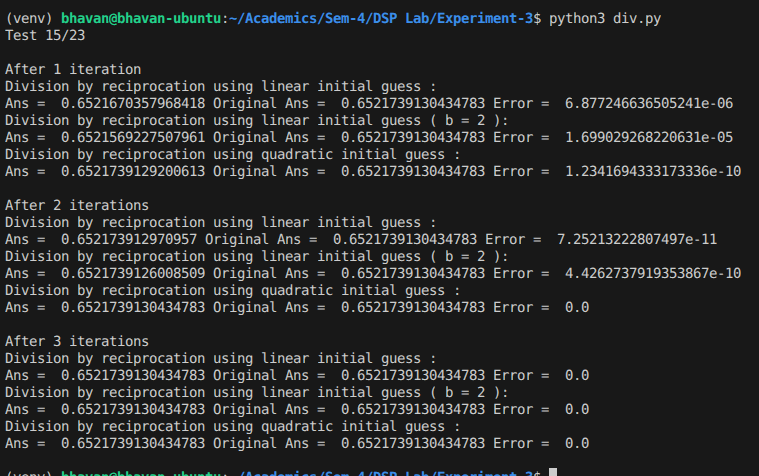
\includegraphics[width=0.75\linewidth]{images/python_error_reduction.png}
    \caption{Python example indicating that error decreases as we increase the number of iterations}
    \label{fig:placeholder}
\end{figure}

\begin{figure}[H]
    \centering
    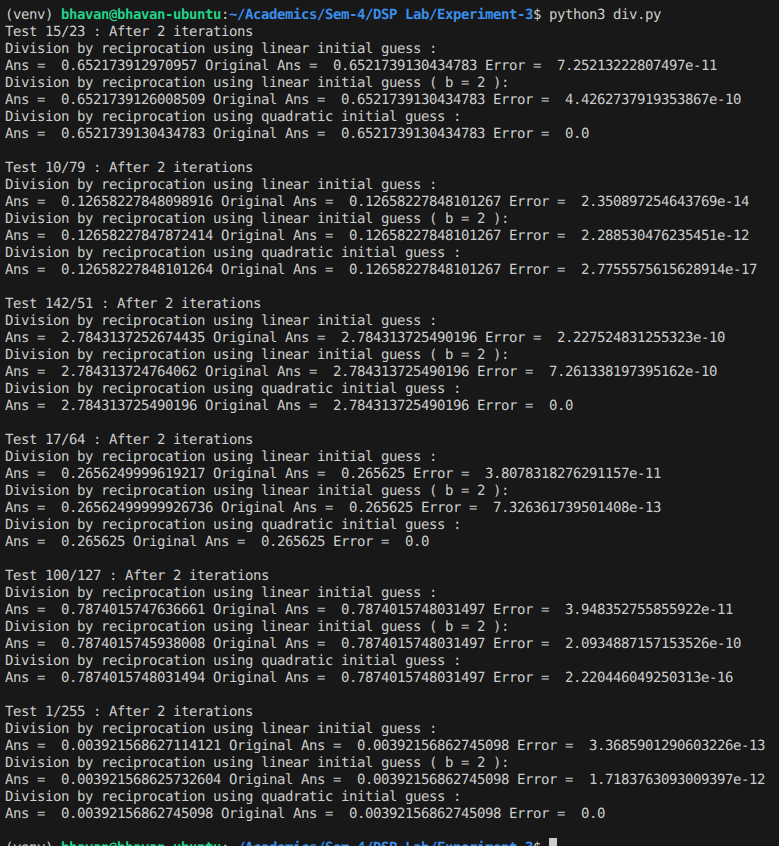
\includegraphics[width=0.75\linewidth]{images/python_errors.png}
    \caption{Python output after 2 iterations}
    \label{fig:placeholder}
\end{figure}


\begin{figure}[H]
    \centering
    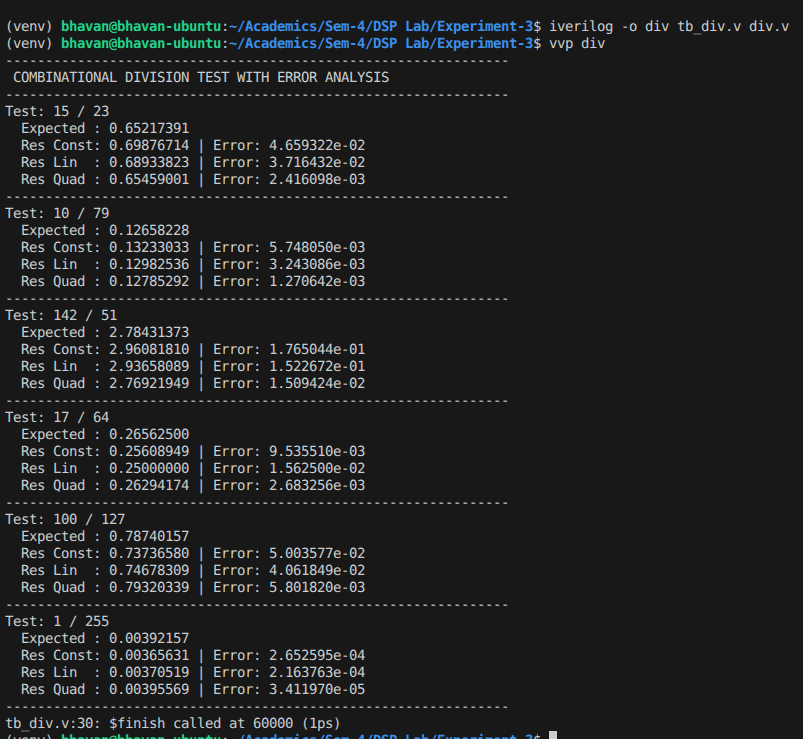
\includegraphics[width=0.75\linewidth]{images/verilog_iter0.png}
    \caption{Verilog - Using the initial guess ( 0 iterations )}
    \label{fig:placeholder}
\end{figure}


\begin{figure}[H]
    \centering
    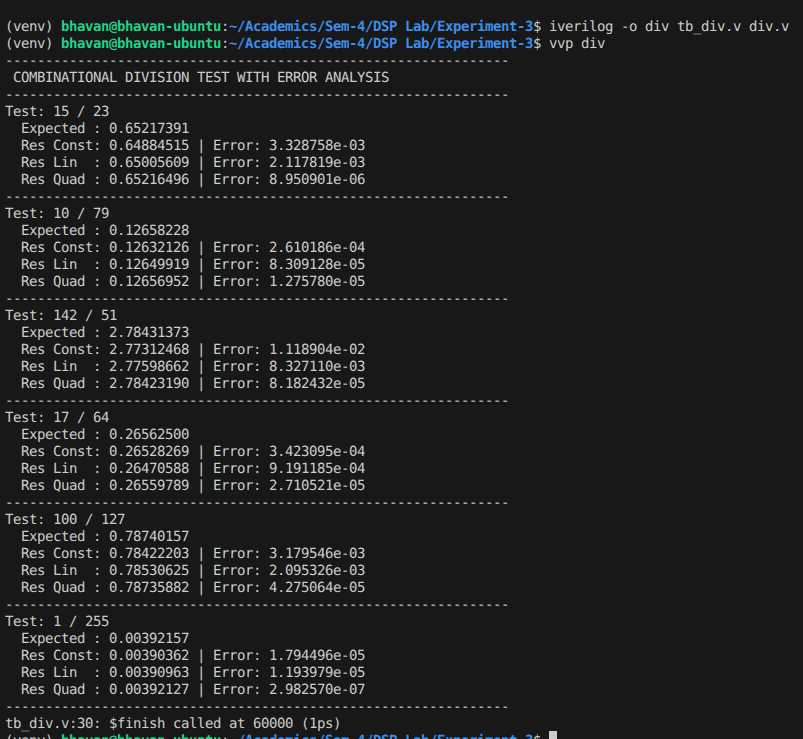
\includegraphics[width=0.75\linewidth]{images/verilog_iter1.png}
    \caption{Verilog - After 1 iteration}
    \label{fig:placeholder}
\end{figure}


\begin{figure}[H]
    \centering
    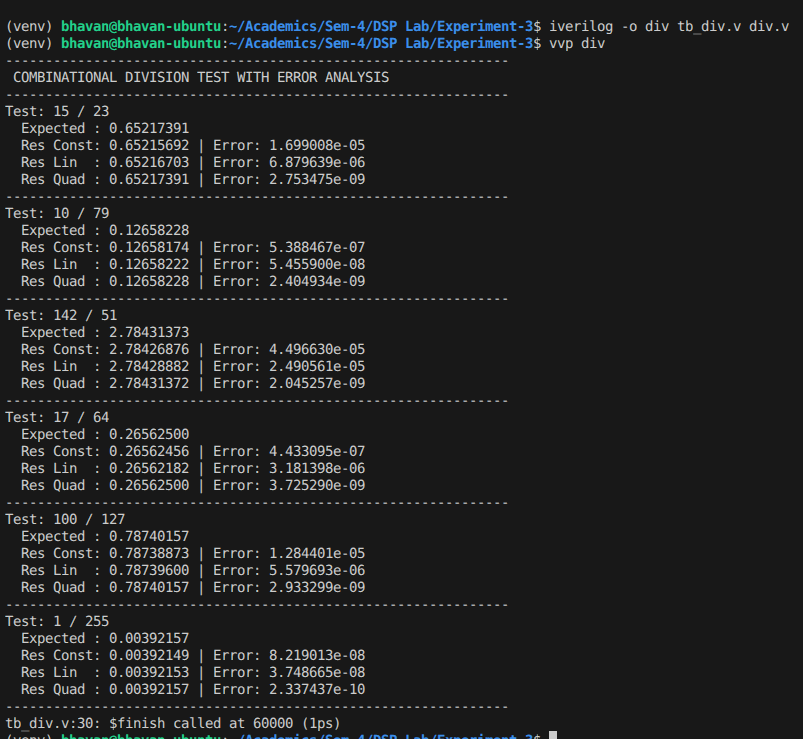
\includegraphics[width=0.75\linewidth]{images/verilog_iter2.png}
    \caption{Verilog - After 2 iterations}
    \label{fig:placeholder}
\end{figure}


\begin{figure}[H]
    \centering
    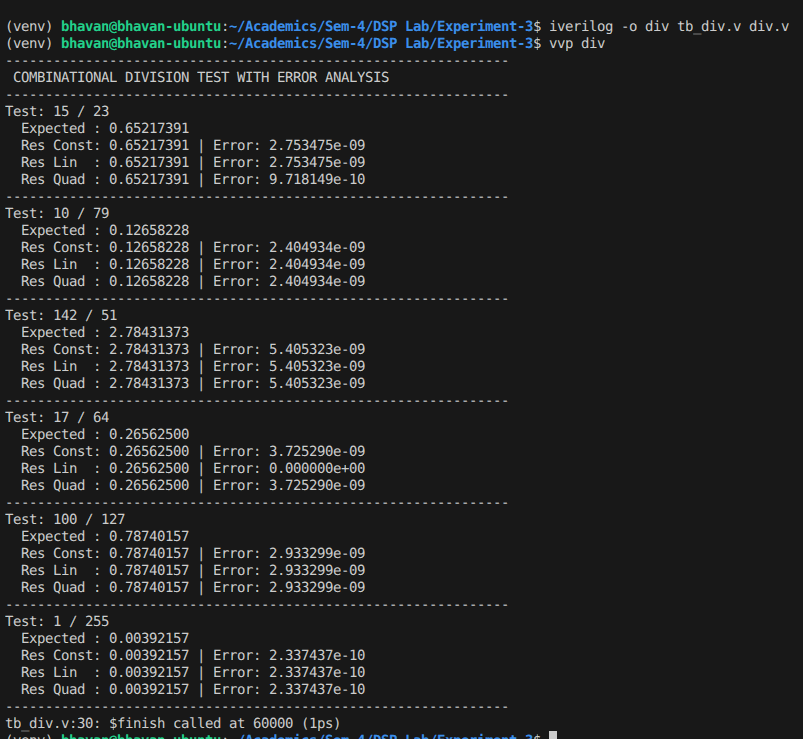
\includegraphics[width=0.75\linewidth]{images/verilog_iter3.png}
    \caption{Verilog - After 3 iterations}
    \label{fig:placeholder}
\end{figure}

\newpage
\section{Observations}

\begin{itemize}
    \item The Verilog simulation results show rapid convergence across successive Newton--Raphson iterations, closely matching the theoretical behavior predicted by the Python reference model.
    \item During the early stages (Iteration 0 and Iteration 1), the quadratic and linear initial guesses exhibit significantly lower initial errors compared to the constrained guess, as expected.
    \item By Iteration 3, the absolute error for all three approximation methods converges to a similar lower bound, typically in the range of $10^{-9}$ to $10^{-10}$.
    \item This error plateau in the Verilog results is caused by the finite precision of the 32-bit Q4.28 fixed-point representation.
    \item The smallest representable fractional value in Q(4,28) format is:
    \[
        2^{-28} \approx 3.72 \times 10^{-9}
    \]
    which defines the theoretical precision limit of the hardware implementation.
    \item In contrast, the Python reference model uses 64-bit double-precision floating-point arithmetic, allowing convergence toward machine epsilon (approximately $10^{-16}$) within the same number of iterations.
     \item The quadratic initial guess requires more hardware but converges in less iterations than the linear guess. This is a trade-off that exists here.
\end{itemize}

\section{Conclusion}
The Newton-Raphson method provides fast quadratic convergence for hardware division via reciprocal computation. Normalizing the denominator to the $[0.5, 1.0)$ interval and applying minimax-optimized initial approximations significantly reduces the required iteration count. Furthermore, the Q(4,28) fixed-point format ensures high numerical precision, achieving absolute errors on the order of $10^{-9}$, while maintaining a fast and resource-efficient hardware datapath.

\end{document}

